\documentclass[aspectratio=43]{beamer}

%%%%%%%%%%%%%%%%%%%%%%%%%%%%%%%%%%%%%%%%%%%%%%%%%%%%%%%%%%%%%%%%%%%%
% über aspectratio kann das Format eingestellt werden. Der Default
% wert ist 43 (4:3, 128mm:96mm). Andere Möglichkeiten sind
% 32 (3:2, 135mm:90mm)
% 54 (5:4, 125mm:100mm)
% 149 (14:9, 14cm:9cm)
% 169 (16:9, 16cm:9cm)
% 1610 (16:10, 16cm:10cm)
% 141 (1.41:1, 148.5mm:105mm, Seitenverhältnis wie bei DIN-A)
%%%%%%%%%%%%%%%%%%%%%%%%%%%%%%%%%%%%%%%%%%%%%%%%%%%%%%%%%%%%%%%%%%%%


\usepackage[T1]{fontenc}
\usepackage[utf8x]{inputenc}
\usepackage[ibycus,ngerman]{babel}
\usepackage{amsfonts,amsmath,amssymb,amsthm}
\usepackage{csquotes}

\usepackage{hyperref}




\usetheme[komms=false]{fbmathematik}

%%%%%%%%%%%%%%%%%%%%%%%%%%%%%%%%%%%%%%%%%%%%%%%%%%%%%%%%%%%
% Schriftfarben:
% tuklblau, tuklrot, warmgrau, kaltgrau;
% abgeschwächte Töne für die obigen Farben und schwarz:
% z.B. tuklblau7 für 70% tuklblau, warmgrau2 für 20%
% warmgrau oder schwarz6 für 60% schwarz,
% jeweils in den Schritten 10%, 20%, 40%, 60%, 70%, 80%;
% violette Schriftfarbe (Felix-Klein) hat den Namen fkz1
% hellviolette FKZ-Variante hat den Namen fkz2;
%%%%%%%%%%%%%%%%%%%%%%%%%%%%%%%%%%%%%%%%%%%%%%%%%%%%%%%%%%%
% Schriftfarben:
% tuklblau, tuklrot, warmgrau, kaltgrau;
% abgeschwächte Töne für die obigen Farben und schwarz:
% z.B. tuklblau7 für 70% tuklblau, warmgrau2 für 20%
% warmgrau oder schwarz6 für 60% schwarz,
% jeweils in den Schritten 10%, 20%, 40%, 60%, 70%, 80%;
% violette Schriftfarbe (Felix-Klein) hat den Namen fkz1
% hellviolette FKZ-Variante hat den Namen fkz2;
% KOMMS: kommsblau, kommsgruen, kommsgrau, kommsblaugrau
%%%%%%%%%%%%%%%%%%%%%%%%%%%%%%%%%%%%%%%%%%%%%%%%%%%%%%%%%%%



\title{Projektvorstellung: Immer der Sonn' entgegen}
\author{Dominik Bendle \and Melissa Hasel \and Thomas Hofmann}
\date{\today}
\institute{TU Kaiserslautern}

\begin{document}
\begin{frame}[plain]

    \Titel{logo}

\end{frame}

\begin{frame}
    \frametitle{Immer der Sonn' entgegen}
    \begin{itemize}
        \item Starten bei Sonnenaufgang, laufen immer in Richtung Sonne und enden bei
            Sonnenuntergang
    \end{itemize}
\end{frame}

\begin{frame}
    \frametitle{Vergleich eigenes \& exaktes Modell}
    \begin{itemize}
        \item Unterschied ist meist vernachlässigbar
        \item auf Straßen können kleine Unterschiede jedoch zu größeren Unterschieden
            führen
    \end{itemize}
\end{frame}

\begin{frame}
    \frametitle{Beispiele}
    \begin{figure}[t]
        \centering
        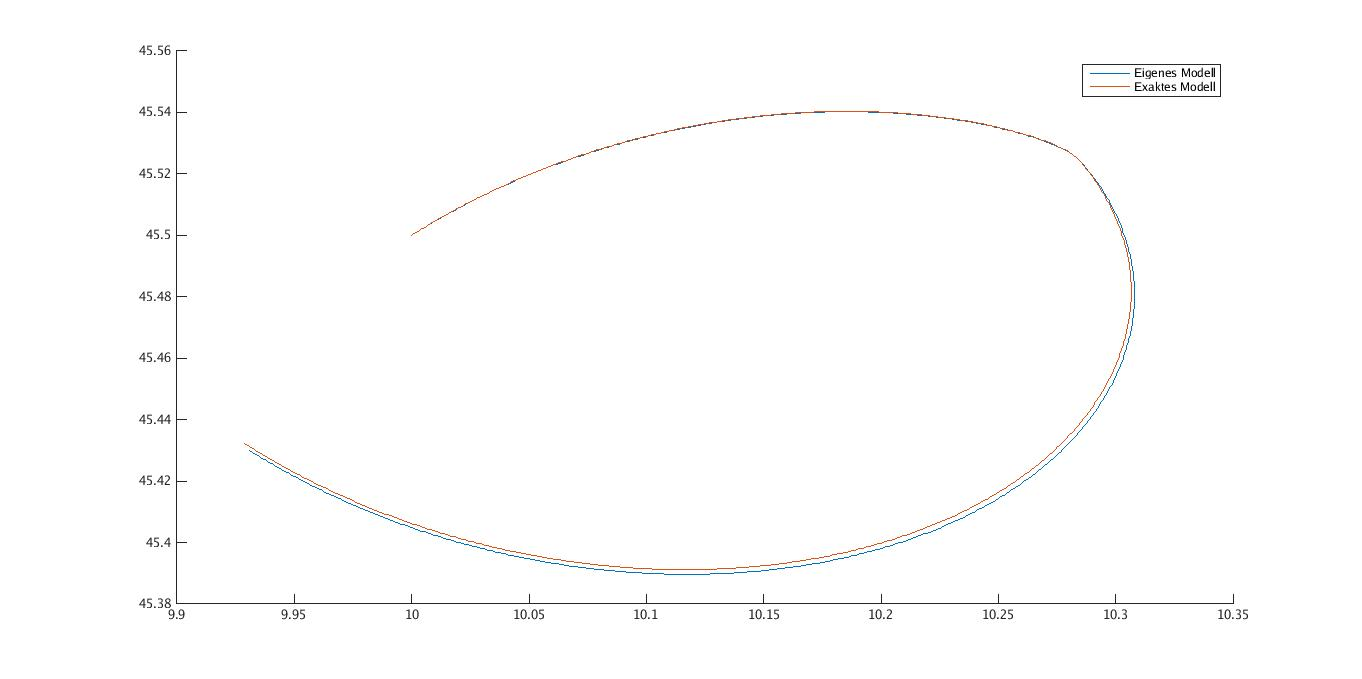
\includegraphics[width=0.95\textwidth]{bilder/hdiffgut.jpg}
        \caption{Einfaches Modell, kein Unterschied}
    \end{figure}
\end{frame}

\begin{frame}
    \frametitle{Beispiele}
    \begin{figure}[t]
        \centering
        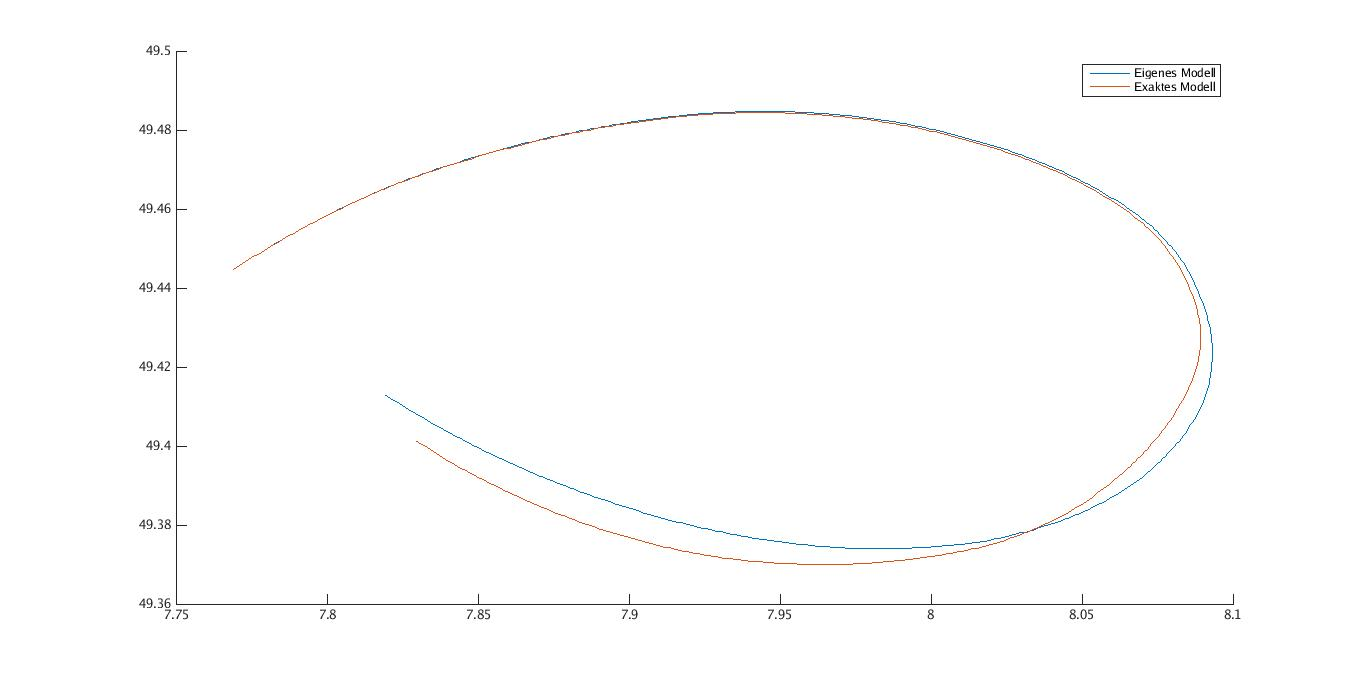
\includegraphics[width=0.95\textwidth]{bilder/hdiffschlecht.jpg}
        \caption{Einfaches Modell, wesentlicher Unterschied}
    \end{figure}
\end{frame}

\begin{frame}
    \frametitle{Beispiele}
    \begin{figure}[t]
        \centering
        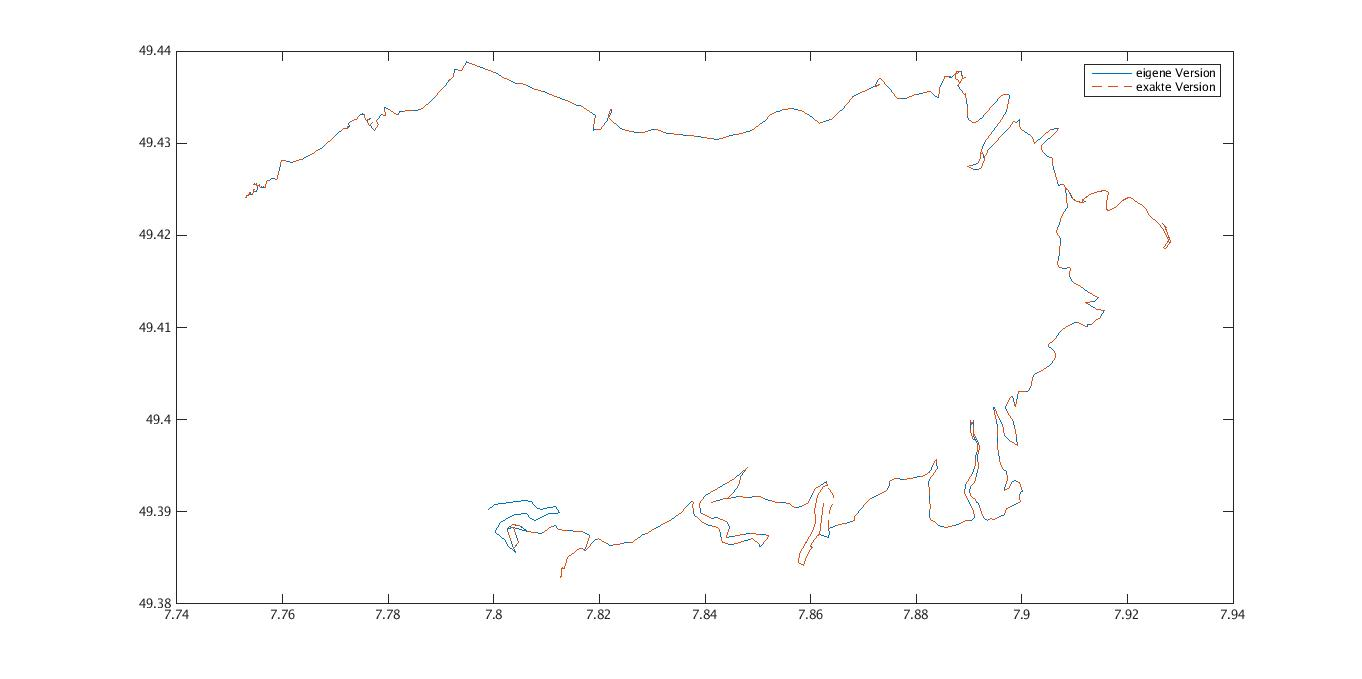
\includegraphics[width=0.95\textwidth]{bilder/kldiff.jpg}
        \caption{Straßendaten, kein Unterschied}
    \end{figure}
\end{frame}

\begin{frame}
    \frametitle{Beispiele}
    \begin{figure}[t]
        \centering
        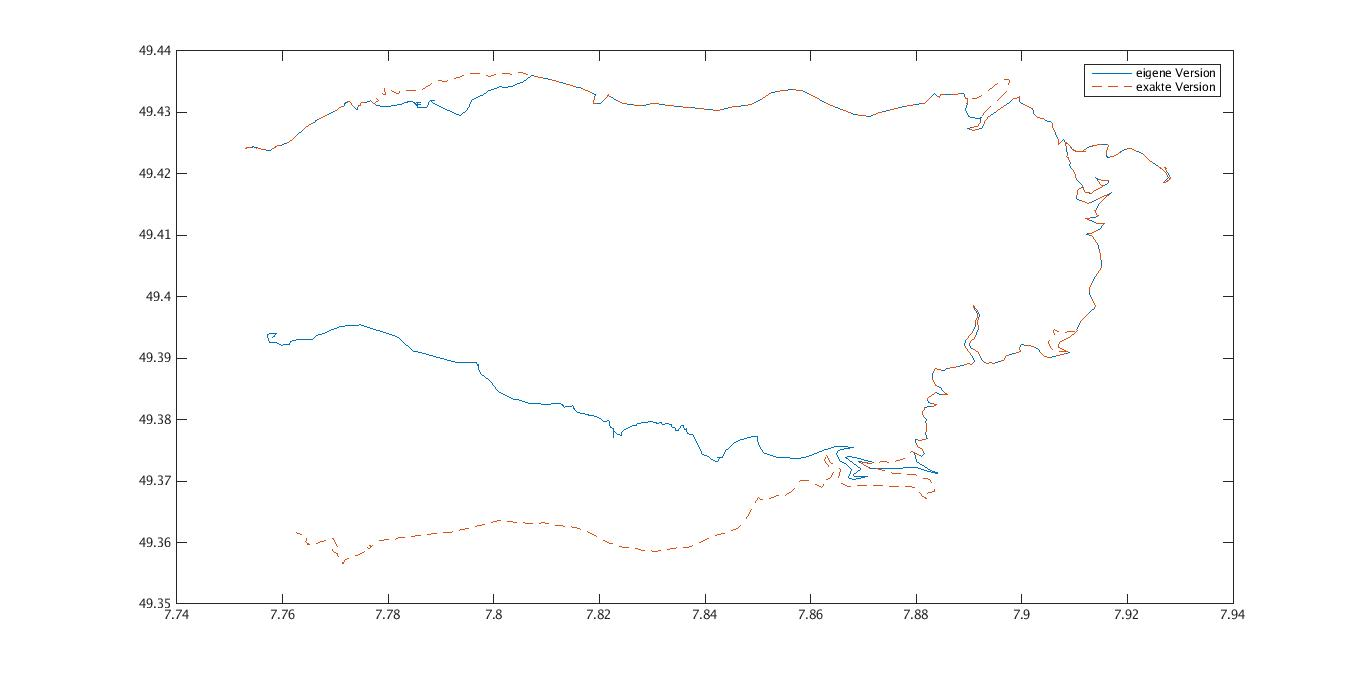
\includegraphics[width=0.95\textwidth]{bilder/kldiffschlecht.jpg}
        \caption{Straßendaten, wesentlicher Unterschied}
    \end{figure}
\end{frame}

\begin{frame}
    \frametitle{Weitere mögliche Features}
    \begin{itemize}
        \item Laufen in Richtung eines beliebigen Punktes
        \item Beliebiger Raumkurve folgen
        \item Immer dem Mond hinterer 
    \end{itemize}
\end{frame}
\end{document}

